\section{Primera parte: amplificador inversor}

Se monta el circuito de la fig. \ref{fig:1:esquema} en una \textit{protoboard}
utilizando resistencias $R_1 = \SI{10}{\kilo\ohm}$, $R_2 = \SI{15}{\kilo\ohm}$ y
$R_3 = \SI{10}{\kilo\ohm}$. Se hace uso de un integrado TL072 como amplificador
operacional, de una fuente partida de \SI{14}{\volt} como su fuente de 
alimentación ($V_{cc}$), y de una pila de $\SI{9}{\volt}$ como $V_1$.
Luego se miden las tensiones $v_i$, $v_o$, $v_{+}$,
$v_{-}$ y $\left(v_{+} - v_{-}\right)$, y se calculan las corrientes que
atraviesan a todas las resistencias para valores de $R_L$ de 1, 10 y
\SI{47}{\kilo\ohm}.

\begin{figure}[H]
    \centering
    \begin{circuitikz}
    \node[op amp] at (0, 0) (opamp) {};

    \draw(opamp.+) -- ++(-0.2, 0) node[label={left:$v_+$}]{}
    to[R=$R_3$] ++(0, -2) coordinate(cg)
    node[ground]{};

    \draw(opamp.-) -- ++(-0.7, 0) node[label={above:$v_-$}]{}
    to[R=$R_1$] ++(-1.5, 0)
    to[short] ++(-0.2, 0) coordinate(ci) node[above]{$v_i$}
    to[battery1, l=$V_1$] (cg -| ci) node[ground]{};

    \draw(opamp.-) -- ++(-0.2, 0)
    to[short, *-] ++(0, 2)
    to[R=$R_2$] ++(2.8, 0) coordinate(co)
    to[short] (opamp.out -| co) coordinate(co1) -- (opamp.out);

    \draw(co1) 
    to[short, *-o] ++(0.4, 0) node[right]{$v_o$};

    \draw(co1)
    to[R=$R_L$] (cg -| co1) node[ground]{};

    \draw(opamp.up) -- ++(0, 0.2) node[vcc]{$+V_{cc}$};
    \draw(opamp.down) -- ++(0, -0.2) node[vee]{$-V_{cc}$};
\end{circuitikz}

    \caption{Esquemático del circuito de la primera parte}
    \label{fig:1:esquema}
\end{figure}

\subsection{Resolución teórica}

Considerando al operacional como un elemento ideal (ver sección \ref{sec:intro})
se sabe que su resistencia de entrada es infinita. Por tal motivo no circulará
corriente a través de la resistencia $R_3$, lo cual implica que no habrá caída
de tensión alguna entre sus terminales. Efectivamente es como tener el circuito
descrito en la sección \ref{sec:intro:opamp-inversor} y por ende se puede usar
la ecuación \ref{ec:intro:opamp-inversor}. Entonces queda:

\begin{equation}
    \label{ec:1-teoria:ganancia}
    A = -\frac{R_2}{R_1}
\end{equation}

\begin{equation}
    \label{ec:1-teoria:err-ganancia}
    \Delta A = \left| - \frac{1}{R_1} \right| \Delta R_2
             + \left| - \frac{R_2}{{R_1}^2} \right| \Delta R_1
\end{equation}

Se observa que el valor de la ganancia \textbf{no depende del valor de la
resistencia de carga}. Considerando que $\Delta R_i = 0.2\,R_i\ \forall\ i$, ya
que los resistores utilizados tienen una tolerancia de $\pm 20\%$, el análisis
anterior resulta en:

\[
    \input{src/1/snippets/ganancia-analitica}
\]

Como puede observarse, el valor de la ganancia no debería verse afectado por el
resistor $R_3$. Esto se debe a la alta resistencia de entrada del operacional
(que de hecho es infinita en este modelo ideal).


\subsection{Simulación con LTSpice}

Se simula el circuito de la fig. \ref{fig:1:esquema} con LTSpice buscando el 
punto de operación (\verb|.op|), como puede verse en la captura de pantalla
de la fig. \ref{fig:1:ltspice}. Los datos obtenidos se encuentran en las tablas
\ref{tab:1:ltspice-tensiones} y \ref{tab:1:ltspice-corrientes}.

Tomando los valores de la tabla \ref{tab:1:ltspice-tensiones} se llega,
mediante la ec. \ref{ec:1-teoria:ganancia}, a un valor de $A = -1.517$ para
todos los casos. Dicho valor concuerda con el análisis teórico de la sección
anterior, aunque su incertidumbre es difícil de estimar.

\begin{figure}[H]
    \centering
    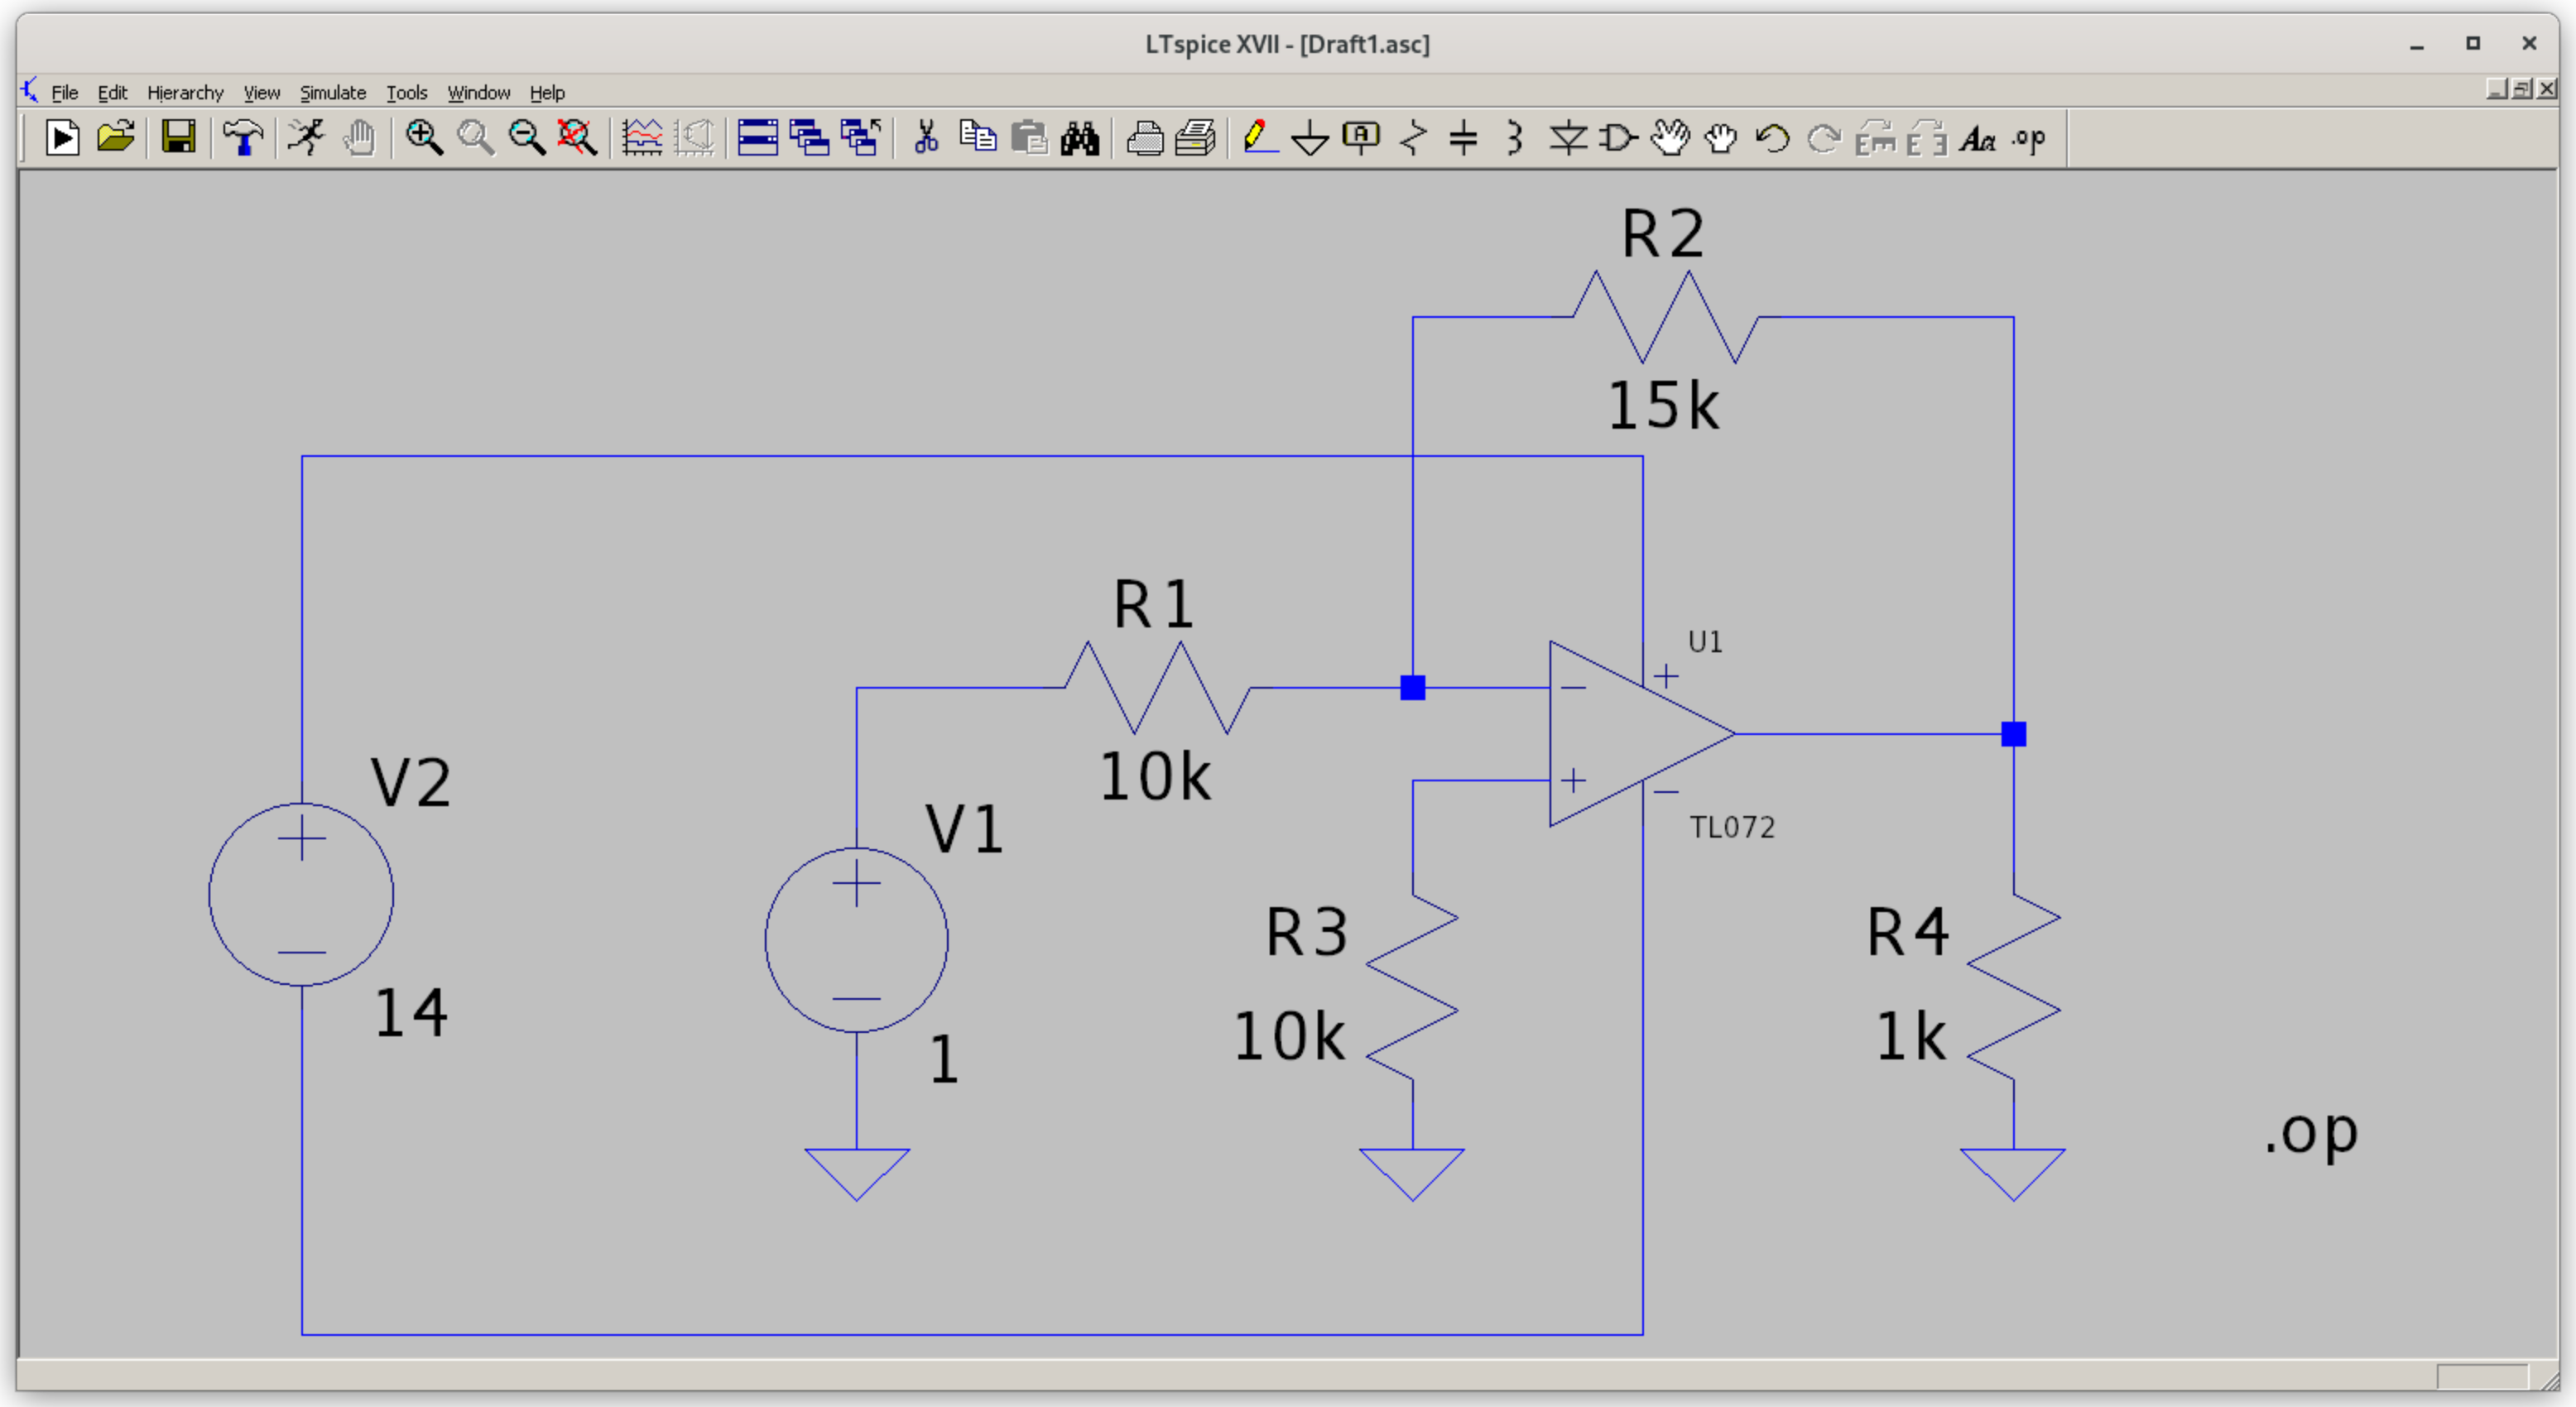
\includegraphics[width=0.8\textwidth]{img/1/ltspice.png}
    \caption{Pantalla de LTSpice}
    \label{fig:1:ltspice}
\end{figure}

\begin{table}[H]
    \centering
    \begin{tabular}{@{}r|rrrr@{}}
    \toprule
    $R_L$ (\si{\kilo\ohm}) & $v_o$ (\si{\volt}) & $v_+$ (\si{\nano\volt}) & 
    $v_-$ (\si{\milli\volt}) & $v_+ - v_-$ (\si{\milli\volt}) \\
    \midrule
    $47$ & $-13.6573$ & $-562.558$ & $-62.9007$ & $62.9001$ \\
    $10$ & $-13.5672$ & $-562.558$ & $-62.8992$ & $62.8986$ \\
     $1$ & $-13.6572$ & $-562.557$ & $-62.8821$ & $62.8815$ \\ \bottomrule
    \end{tabular}
    \caption{Tensiones según LTSpice ($v_i = \SI{9.00}{\volt}$)}
    \label{tab:1:ltspice-tensiones}
\end{table}

\begin{table}[H]
    \centering
    \begin{tabular}{@{}r|rrrr@{}}
        \toprule
        $R_L$ (\si{\kilo\ohm}) & $I_{R_1}$ (\si{\milli\ampere}) &
        $I_{R_2}$ (\si{\milli\ampere}) & $I_{R_3}$ (\si{\pico\ampere}) &
        $I_{R_L}$ (\si{\milli\ampere}) \\
        \midrule
        $47$ & $0.29058$ & $0.906290$ & $56.2558$ & $0.29058$ \\
        $10$ & $1.36572$ & $0.906290$ & $56.2558$ & $1.36572$ \\
         $1$ & $13.6572$ & $0.906288$ & $56.2557$ & $13.6572$ \\ \bottomrule
        \end{tabular}
        \caption{Corrientes según LTSpice}
        \label{tab:1:ltspice-corrientes}
\end{table}



\subsection{Datos obtenidos}

Se miden los siguientes valores de resistencias:

\begin{itemize}
        \input{src/1/snippets/resistencias}
\end{itemize}

Los valores medidos de $R_L$, comparados con sus valores nominales, se encuentran en la tabla \ref{tab:1-datos:resistencias-l}.

También se toman mediciones de las distintas tensiones presentes en el circuito (tablas \ref{tab:1-datos:tensiones-1} y \ref{tab:1-datos:tensiones-2}) que son utilizadas para calcular las corrientes que circulan por cada resistor y cuyos valores se encuentran en la tabla \ref{tab:1-datos:corrientes}.

\begin{table}[H]
    \centering
    \begin{tabular}{@{}rr@{}}
        \toprule
        $R_L$ (nominal, \si{\kilo\ohm}) & $R_L$ (medido, \si{\kilo\ohm})  \\
        \midrule
        \input{src/1/tables/resistencias-l}
    \end{tabular}
    \caption{Valores medidos de $R_L$}
    \label{tab:1-datos:resistencias-l}
\end{table}

\begin{table}[H]
    \centering
    \begin{tabular}{@{}rrrrrr@{}}
        \toprule
        $R_L$ (\si{\kilo\ohm}) & $v_i$ (\si{\volt}) & $v_o$ (\si{\volt}) & 
            $v_+$ (\si{\milli\volt}) & $v_-$ (\si{\milli\volt}) &
            $v_+ - v_-$ (\si{\milli\volt}) \\
        \midrule
        \input{src/1/tables/tensiones-1}
    \end{tabular}
    \caption{Tensiones medidas en el circuito (parte 1)}
    \label{tab:1-datos:tensiones-1}
\end{table}

\begin{table}[H]
    \centering
    \begin{tabular}{@{}rrrrrr@{}}
        \toprule
        $R_L$ (\si{\kilo\ohm}) & $V_{R_1}$ (\si{\volt}) & $V_{R_2}$ (\si{\volt})& $V_{R_3}$ (\si{\milli\volt}) & $V_{R_L}$ (\si{\volt}) \\
        \midrule
        \input{src/1/tables/tensiones-2}
    \end{tabular}
    \caption{Tensiones medidas en el circuito (parte 2)}
    \label{tab:1-datos:tensiones-2}
\end{table}

\begin{table}[H]
    \centering
    \begin{tabular}{@{}rrrrr@{}}
        \toprule
        $R_L$ (\si{\kilo\ohm}) & $I_{R_1}$ (\si{\milli\ampere}) & $I_{R_2}$ (\si{\milli\ampere}) & $I_{R_3}$ (\si{\nano\ampere}) & $I_{R_L}$ (\si{\milli\ampere}) \\
        \midrule
        \input{src/1/tables/corrientes}
    \end{tabular}
    \caption{Corrientes calculadas en el circuito}
    \label{tab:1-datos:corrientes}
\end{table}

La ganancia del operacional puede calcularse experimentalmente con las
ecuaciones \ref{ec:1-teoria:ganancia-experimental} y
\ref{ec:1-teoria:err-ganancia-experimental}. Los resultados de esta
operación se encuentran en la tabla \ref{tab:1-teoria:ganancia-experimental}.

\begin{equation}
    \label{ec:1-teoria:ganancia-experimental}
    A = \frac{v_o}{v_i}
\end{equation}

\begin{equation}
    \label{ec:1-teoria:err-ganancia-experimental}
    \Delta A = \left| \frac{1}{v_i} \right| \Delta v_o + \left| -\frac{v_o}{{v_i}^2} \right| \Delta v_i
\end{equation}

\begin{table}[H]
    \centering
    \begin{tabular}{@{}rr@{}}
        \toprule
        $R_L$ (\si{\kilo\ohm}) & $A$ \\
        \midrule
        \input{src/1/tables/ganancia-experimental}
    \end{tabular}
    \caption{Valores experimentales de ganancia}
    \label{tab:1-teoria:ganancia-experimental}
\end{table}

Teniendo $R_L = \SI{1}{\kilo\ohm}$ se reemplaza la pila de \SI{9}{\volt} por
un generador de funciones configurado para entregar una señal senoidal de
\SI{2}{\volt} de amplitud pico-a-pico y frecuencia $f = \SI{1}{\kilo\hertz}$.
Se conecta también un osciloscopio, cuya pantalla
se muestra en la fig. \ref{fig:1-datos:osciloscopio}. Se observa que la señal
de salida tiene una amplitud muy cercana a la de entrada (\SI{1.02}{\volt} vs.
\SI{1.08}{\volt}), y que se encuentra desfasada en unos \SI{90}{\degree}.

\begin{figure}[H]
    \centering
    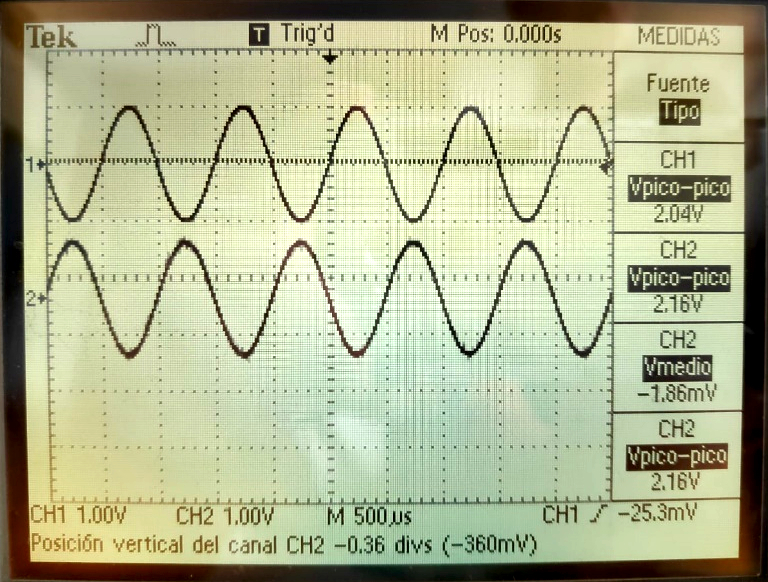
\includegraphics[width=0.8\textwidth]{img/1/osciloscopio-1.jpg}
    \caption{Pantalla del osciloscopio. Se muestran la señal de entrada
        (arriba, canal 1) y la de salida (abajo, canal 2).}
    \label{fig:1-datos:osciloscopio}
\end{figure}


\subsection{Análisis de datos}

El gráfico de la fig. \ref{fig:1-analisis:ganancia} muestra una comparación
entre el valor de ganancia teórico (calculado con las ecuaciones 
\ref{ec:1-teoria:ganancia} y \ref{ec:1-teoria:err-ganancia}) y aquellos 
medidos en la práctica para los distintos valores de resistencia. Como puede
observarse, todos los valores de ganancia medidos caen cómodamente dentro
del margen de error previsto. Esto sugiere que las ecuaciones de ganancia
que se utilizaron para la configuración inversora del amplificador operacional
permiten obtener una buena aproximación al funcionamiento real del circuito.

\begin{figure}[H]
    \centering
    \input{img/1/ganancia.tikz}
    \caption{Valores de ganancia medidos vs. teóricos}
    \label{fig:1-analisis:ganancia}
\end{figure}

Dado que los valores medidos de tensión en la terminal no inversora son
mayores que $0$ en dos de los tres casos estudiados\footnote{Es altamente
probable que $v_+$ estuviera en el orden de los \si{\micro\volt}, en cuyo
caso nos fue imposible medir con el multímetro del que disponíamos.}, se
comprueba la explicación ofrecida en la sección \ref{sec:1-teoria} sobre la
utilización del resistor $R_3$. Si la resistencia de entrada del operacional
fuera infinita, esta tensión sería 0.


% \subsection{Análisis de datos}

La fig. \ref{fig:1-analisis:ganancia} compara la ganancia teórica con los valores obtenidos en la práctica.

\begin{figure}[H]
    \includegraphics[width=\textwidth]{img/1-analisis-ganancia.eps}
    \caption{Ganancia teórica vs. ganancia experimental}
    \label{fig:1-analisis:ganancia}
\end{figure}

